\documentclass{article}

%\usepackage{mathtools}
\usepackage{amsfonts}
\usepackage[spanish,mexico]{babel}
\usepackage[utf8]{inputenc}
\usepackage{graphicx}
\usepackage{booktabs}
\usepackage{url}
\usepackage{listings}%http://www.tex.ac.uk/FAQ-codelist.html
\lstset{language=Python}
\graphicspath{ {img/} }
%\usepackage{enumitem}
%\usepackage{tikz}

\title{Representación mediante grafos de un problema de asignación de horarios}
\author{José Alberto Benavides Vázquez}
\date{\today}

\begin{document}

  \maketitle

  \section{Introducción}

  Los algoritmos de Floyd-Warshall y Ford-Fulkerson se utilizan en teoría de grafos para realizar mediciones de flujos a grafos ponderados. \textbf{Floyd-Warshall} calcula el camino más corto entre todos los pares de vértices, mientras que \textbf{Ford-Fulkerson} se utiliza para encontrar el máximo flujo que puede correr entre un nodo de inicio y uno de fin dados. Los nodos de inicio y fin de este segundo algoritmo se suelen denotar por $s$ y $t$ respectivamente.

  Este par de algoritmos se implementaron en un programa capaz de crear nodos, conectarlos y asignarles pesos y direcciones a las aristas así generadas. Este programa se halla alojado en \url{https://github.com/jbenavidesv87/FlujoRedes}.Se mostrará a continuación la explicación de dichos algoritmos además de ejecutarlos con un ejemplo para mayor claridad.

  \section{Teoría y ejemplos}
  Tanto el algoritmo de Floyd-Warshall como el de Ford-Fulkerson toman un grafo previamente definido con al menos dos nodos conectados entre sí por una arista ponderada. Para demostrar el uso y funcionalidad de estos algoritmos, se construyó a manera de ejemplo un grafo $G$ no dirigido con cuatro nodos $a, b, c, d$, con aristas ponderadas como los mostrados en la figura \ref{fig:ejemplo} (p. \pageref{fig:ejemplo}).

  \begin{figure}[h]
    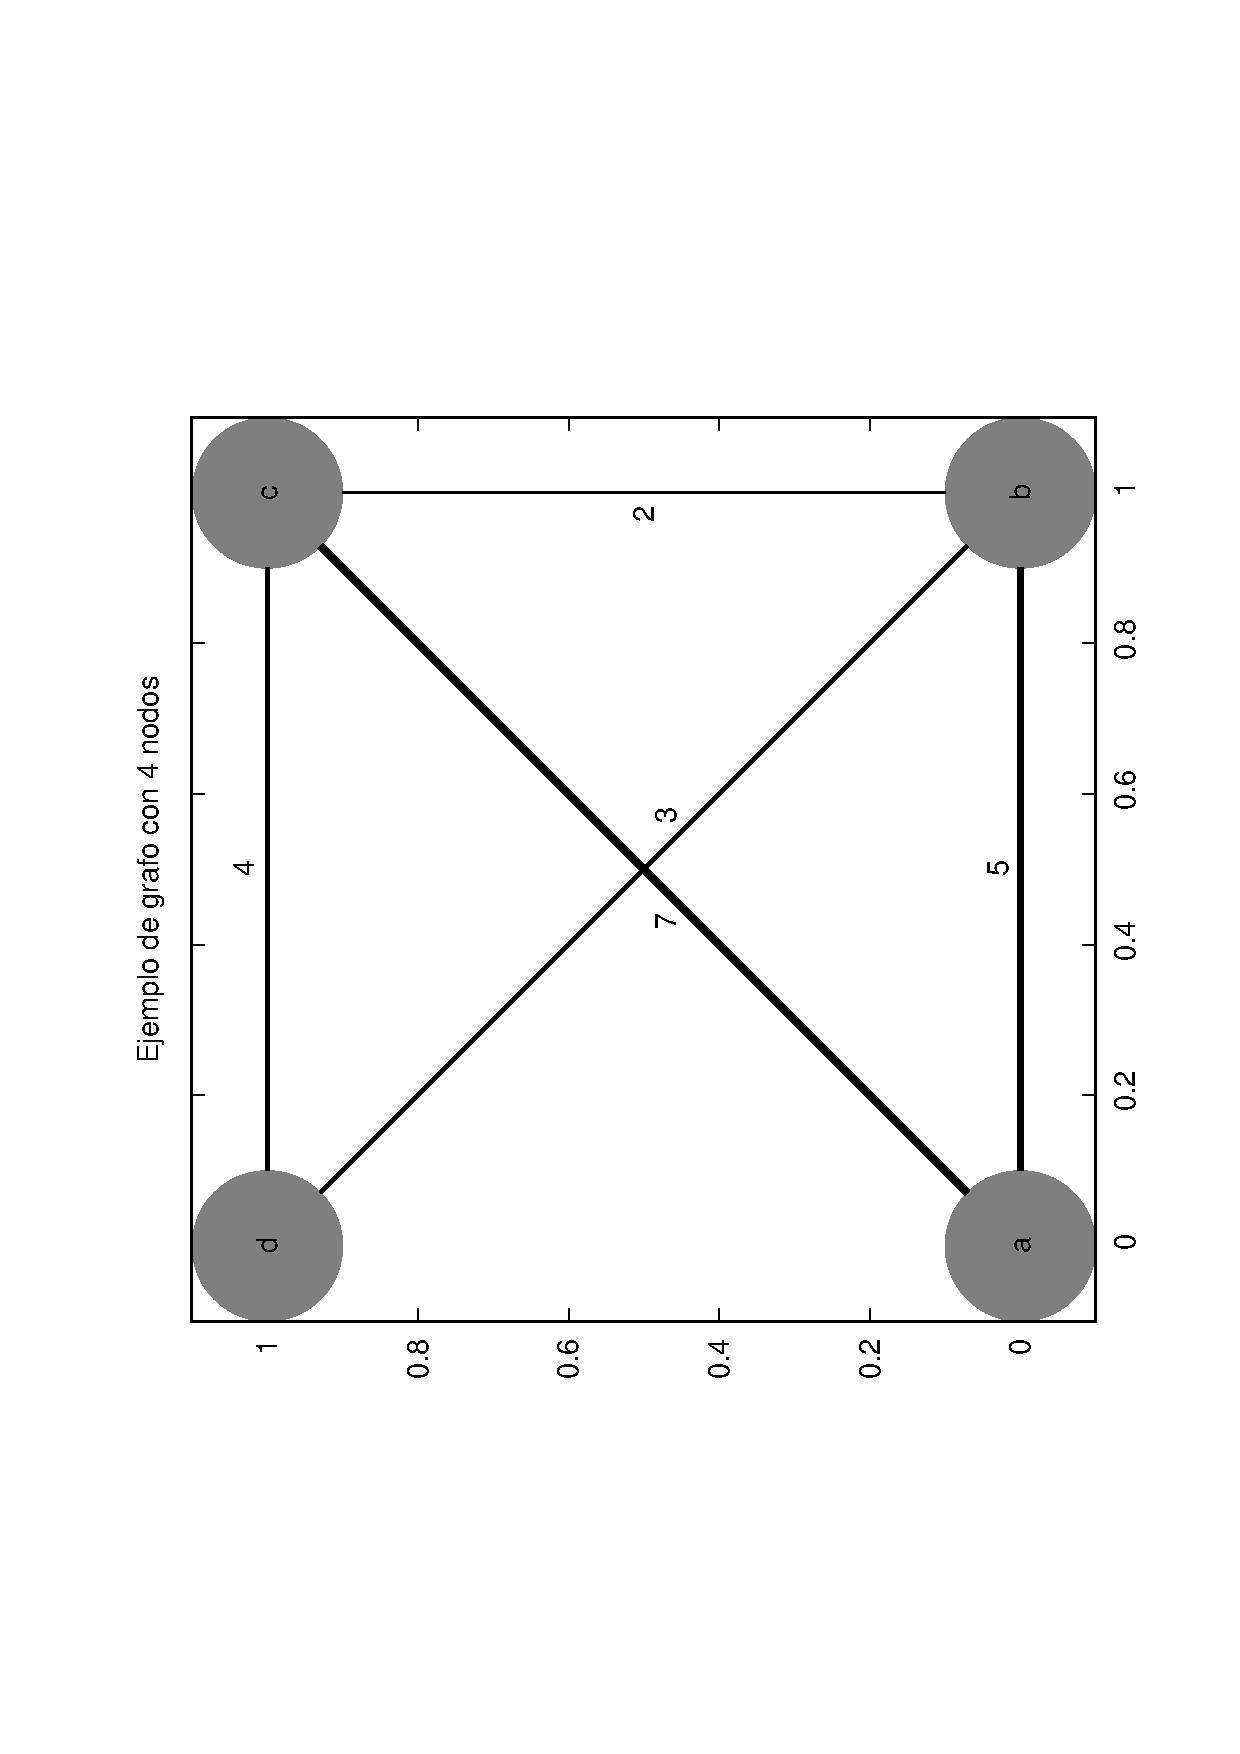
\includegraphics[width=0.7\textwidth, angle=-90]{ejemplo} % https://tex.stackexchange.com/questions/120117/how-to-rotate-eps-file
    \centering
    \caption{Grafo $G$ ponderado con 4 nodos $a, b, c, d$ que se usará como ejemplo para probar el funcionamiento de los algoritmos de Floyd-Warshall y Ford-Fulkerson.}
    \label{fig:ejemplo}
  \end{figure}

  % https://www.youtube.com/watch?v=4OQeCuLYj-4&t=186s
  Tras correr el algoritmo de Floyd-Warshal se obtuvieron, para cada par de nodos, el camino más corto entre todos los nodos del grafo. La distancia de estos caminos se calcula a partir de la suma de los pesos de las aristas que conectan a los nodos entre sí. En cada iteración, se exploran todos los caminos que van desde un nodo inicial hasta uno de destino. Se dice que un camino es mejor que otro cuando se encuentra un camino cuya distancia es menor a una existente (si no hay una distancia previamente almacenada, entonces se toma la primer distancia registrada como la mejor). Al final, el algoritmo regresa una lista de las mejores distancias entre todos los nodos. Para este ejemplo construido, la lista se puede consultar en el cuadro \ref{cuadro:floyd-ejemplo} (p. \pageref{cuadro:floyd-ejemplo}).

  \begin{table}[]
  \centering
  \caption{Camino más corto entre todos los pares de nodos, denotados por cada iteración como nodo inicial $s$ y nodo final $t$, para el grafo $G$ construido a manera de ejemplo inicial.}
  \label{cuadro:floyd-ejemplo}
  \begin{tabular}{@{}ccc@{}}
  \toprule
  \textbf{Nodo inicial $s$} & \textbf{Nodo final $t$} & \textbf{Camino más corto} \\ \midrule
  a & a & 0 \\ \midrule
  a & c & 7 \\ \midrule
  a & b & 5 \\ \midrule
  b & b & 0 \\ \midrule
  b & a & 5 \\ \midrule
  b & d & 3 \\ \midrule
  b & c & 2 \\ \midrule
  c & c & 0 \\ \midrule
  c & a & 7 \\ \midrule
  c & d & 4 \\ \midrule
  c & b & 2 \\ \midrule
  d & d & 0 \\ \midrule
  d & c & 4 \\ \midrule
  d & b & 3 \\ \midrule
  a & d & 8 \\ \midrule
  d & a & 8 \\ \bottomrule
  \end{tabular}
  \end{table}

  %https://www.youtube.com/watch?v=Tl90tNtKvxs
  El máximo flujo entre dos nodos se calcula con el algoritmo de Ford-Fulkerson. Este algoritmo consiste en recorrer todos los caminos que van desde un nodo inicial $s$ hasta uno final $f$, tomando como limitante el peso mínimo entre los pesos de los arcos que constituyen cada camino. Ese peso limitante indica el máximo flujo que podría soportar dicho camino. Cada iteración, se actualiza el grafo en el sentido en que se resta al peso de cada arco del camino elegido, el peso del camino mínimo. Cada iteración posterior, eligirá caminos en los que todos sus arcos posean capacidad disponible y se repite el proceso. Cuando no haya más caminos con arcos que tengan capacidades disponibles, se suman los pesos actualizados del grafo resultante, camino por camino, y se obtiene de su suma el máximo flujo del nodo $s$ al $t$. Del ejemplo graficado en la figura figura \ref{fig:ejemplo} (p. \pageref{fig:ejemplo}) se calculó el flujo máximo entre los nodos $a$ y $b$, obteniendo por resultado $10$; y entre los nodos $a$ y $d$, $7$.

  Ahora, para mostrar el funcionamiento en un grafo dirigido, estos mismos algoritmos se correrá con el mismo grafo, pero dirigido, tal como se muestra en la figura \ref{fig:ejemploDirigido} (p. \pageref{fig:ejemploDirigido}). A este nuevo grafo se le llamará $H$.

  \begin{figure}[h]
    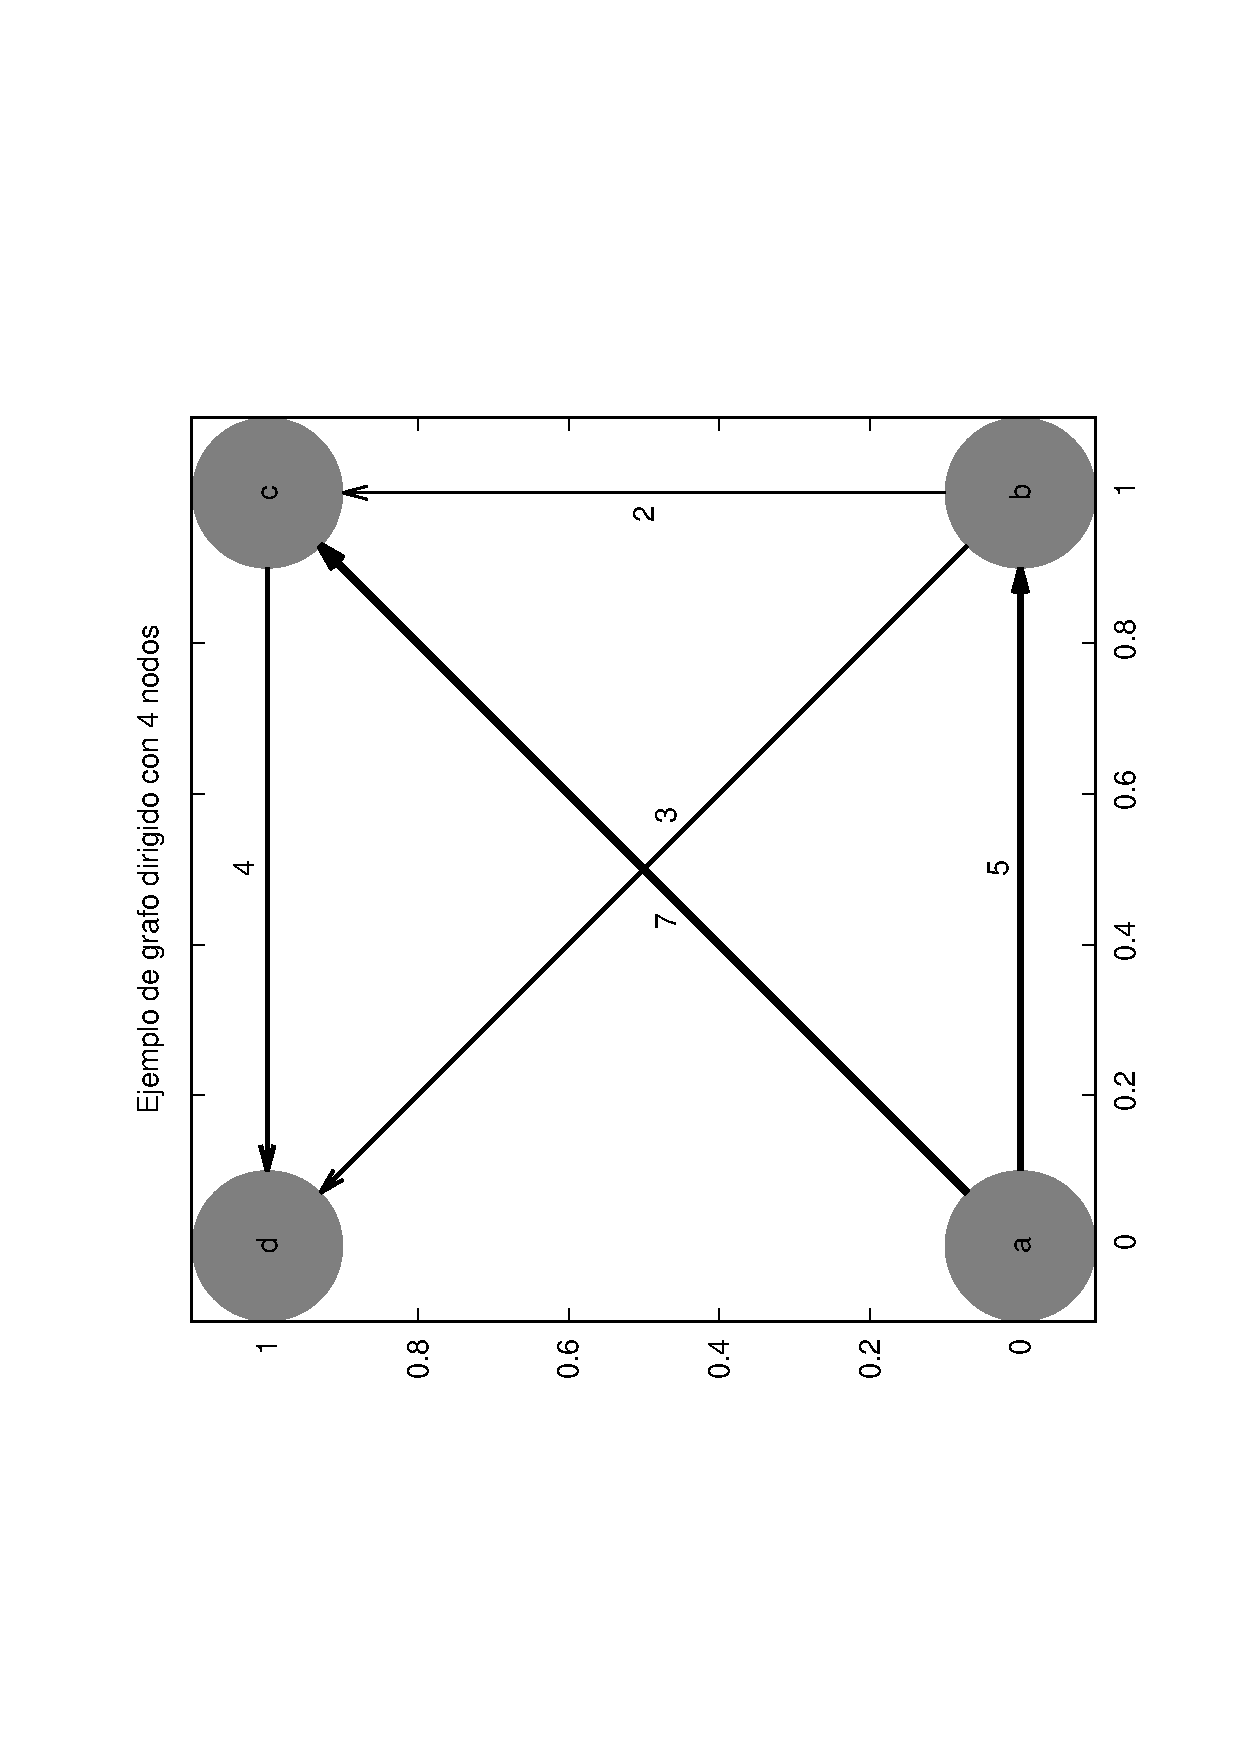
\includegraphics[width=0.7\textwidth, angle=-90]{ejemploDirigido} % https://tex.stackexchange.com/questions/120117/how-to-rotate-eps-file
    \centering
    \caption{Grafo $H$ ponderado y dirigido con 4 nodos $a, b, c, d$ que se usará como ejemplo para probar el funcionamiento de los algoritmos de Floyd-Warshall y Ford-Fulkerson.}
    \label{fig:ejemploDirigido}
  \end{figure}

  Tras correr el algoritmo de Floyd-Warshall sobre el grafo $H$ se obtienen los caminos más cortos mostrados en el cuadro \ref{cuadro:floyd-ejemploDirigido} (\pageref{cuadro:floyd-ejemploDirigido}).

  \begin{table}[]
  \centering
  \caption{Camino más corto entre todos los pares de nodos, denotados por cada iteración como nodo inicial $s$ y nodo final $t$, para el grafo $H$ construido a manera de ejemplo para nodos dirigidos.}
  \label{cuadro:floyd-ejemploDirigido}
  \begin{tabular}{@{}ccc@{}}
  \toprule
  \textbf{Nodo inicial $s$} & \textbf{Nodo final $t$} & \textbf{Camino más corto} \\ \midrule
  a & a & 0 \\ \midrule
  a & c & 7 \\ \midrule
  a & b & 5 \\ \midrule
  b & b & 0 \\ \midrule
  b & c & 2 \\ \midrule
  b & d & 3 \\ \midrule
  c & c & 0 \\ \midrule
  c & d & 4 \\ \midrule
  d & d & 0 \\ \midrule
  a & d & 8 \\ \bottomrule
  \end{tabular}
  \end{table}

  Por su parte, el algoritmo de Ford-Fulkerson en el grafo $H$, da por resultado $5$ del nodo $a$ al $b$; y $7$ del nodo $a$ al $d$.

  Este par de ejemplos están contenidos en un mismo código que se puede encontrar comentado en \url{https://github.com/jbenavidesv87/FlujoRedes/blob/master/ejemplos/05FloydWarshall/main.py}.

  En la siguiente sección, se estudiará el tiempo de ejecución que toma correr cada algoritmo con diferentes tamaños de grafos.

  \section{Tiempos de ejecución}

  Para medir los tiempos de ejecución se realizó un programa que generaba nueve grafos dirigidos con una cantidad de nodos igual a las siguientes potencias de $2$: $2$, $4$, $8$, $16$, $32$, $64$, $128$ y $256$. A cada uno de estos grafos se les efectuó la siguiente serie de acciones:

  \begin{enumerate}
    \item Se crearon $n$ nodos correspondientes a la potencia del grafo en turno.
    \item A cada nodo se le asignó una posición al azar en un espacio unitario bidimensional.
    \item Se calculó la cantidad total de aristas que se podrían establecer entre todas las parejas de nodos, como $t = n (n - 1)$.
    \item Se crearon un total de $\mathrm{techo}(0.1 t)$ aristas entre parejas de nodos elegidos al azar, cuidando que no se repitieran vecinos.
    \item Se calculó el tiempo de ejecución del algoritmo de Floyd-Warshal.
    \item Se eligió al azar una pareja de nodos distintos que sirvieron de base para correr el algoritmo de Ford-Fulkerson y se midió el tiempo que tomó arrojar un resultado.
  \end{enumerate}

  Esta serie de acciones ejecutadas por cada uno de los nueve grafos se repitió veinte veces. Se obtuvieron como resultado grafos como el que se muestra en la figura \ref{fig:16} (\pageref{fig:16}). Para grafos con tamaños menores a $64$ nodos, el tiempo de ejecución del algoritmo de Floyd-Warshal es menor a un segundo, mientras que para grafos de $256$ nodos, se alcanzan tiempos que rondan los once segundos. Los tiempos de corrida del algoritmo de Ford-Fulkerson tienen tiempos menores a un segundo en grafos de $32$, mientras que para grafos de $128$ nodos o superiores, los tiempos podrían sobrepasar el minuto, habiéndose registrado tiempos de hasta $45$ minutos para grafos con $256$ nodos. Suponemos que estos tiempos tan dilatados en comparación con el resto responden a que se eligen al azar grafos muy distantes y con una gran variedad de caminos entre sí. Investigar este comportamiento resultaría interesante pero se escapa de los alcances de este reporte, por lo que se propone como trabajo futuro.

  \begin{figure}[h]
    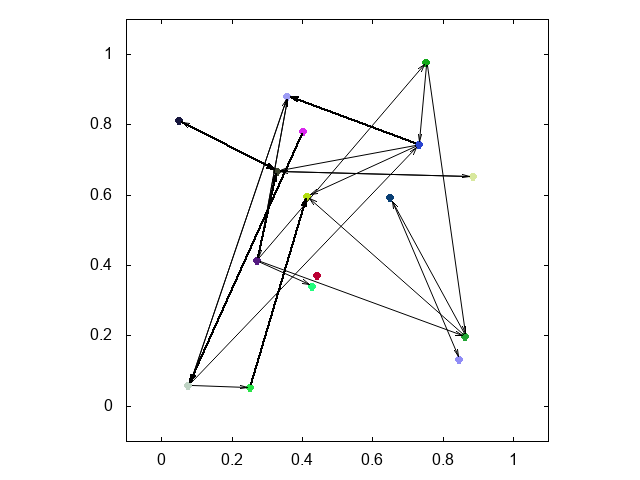
\includegraphics[width=0.7\textwidth]{16} % https://tex.stackexchange.com/questions/120117/how-to-rotate-eps-file
    \centering
    \caption{Ejemplo de grafo de 16 nodos con $24$ arcos, equivalentes a un $10 \%$ del total de arcos posibles, es decir $16 \cdot 15 = 240$ arcos dirigidos posibles.}
    \label{fig:boxplotFord}
  \end{figure}

  Los tiempos registrados para el algoritmo de Floyd-Warshall han sido representados en escala logarítmica y por cantidad de nodos en diagramas de caja y bigotes en la figura \ref{fig:boxplotFloyd} (\pageref{fig:boxplotFloyd}), mientras que para el algoritmo de Ford-Warshall puede consultarse la figura \ref{fig:boxplotFord} (\pageref{fig:boxplotFord}).

  \begin{figure}[h]
    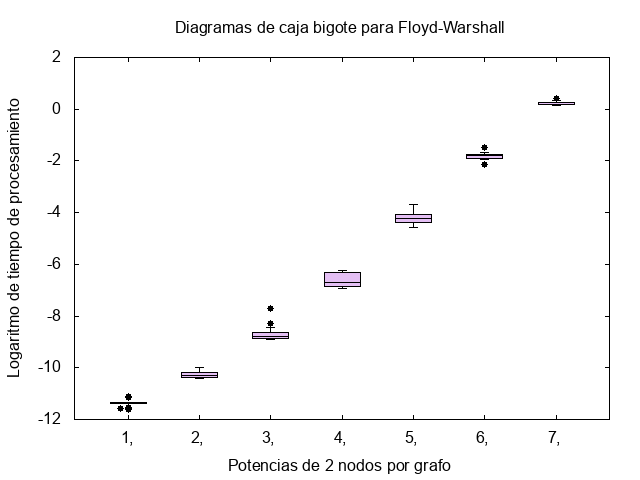
\includegraphics[width=0.7\textwidth]{boxplotFloyd} % https://tex.stackexchange.com/questions/120117/how-to-rotate-eps-file
    \centering
    \caption{Diagrama de caja y bigotes de los tiempos en segundos en escala logarítmica de ejecución del algoritmo de Floyd-Warshall de los grupos de grafos generados al azar.}
    \label{fig:boxplotFloyd}
  \end{figure}

  \begin{figure}[h]
    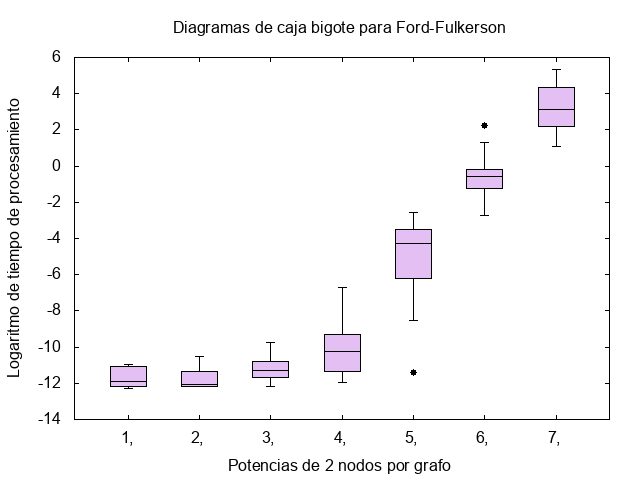
\includegraphics[width=0.7\textwidth]{boxplotFord} % https://tex.stackexchange.com/questions/120117/how-to-rotate-eps-file
    \centering
    \caption{Diagrama de caja y bigotes de los tiempos en segundos en escala logarítmica de ejecución del algoritmo de Ford-Fulkerson de los grupos de grafos generados al azar.}
    \label{fig:boxplotFord}
  \end{figure}

  %\bibliography{biblio}{}
  %\bibliographystyle{plain}

\end{document}
